\section{Couette flow with chain molecules}
A Couette flow system was simulated with two walls moving in opposite directions at velocity $v_{wall} = 5$. The system contained $42$ chain molecules of structure $A-A-B-B-B-B-B$ along with fluid particles. Bond parameters were $K_S = 100$ and $r_S = 0.1$, and conservative force coefficients were set according to the assignment matrix.
\begin{figure}[H]
	\begin{center}
		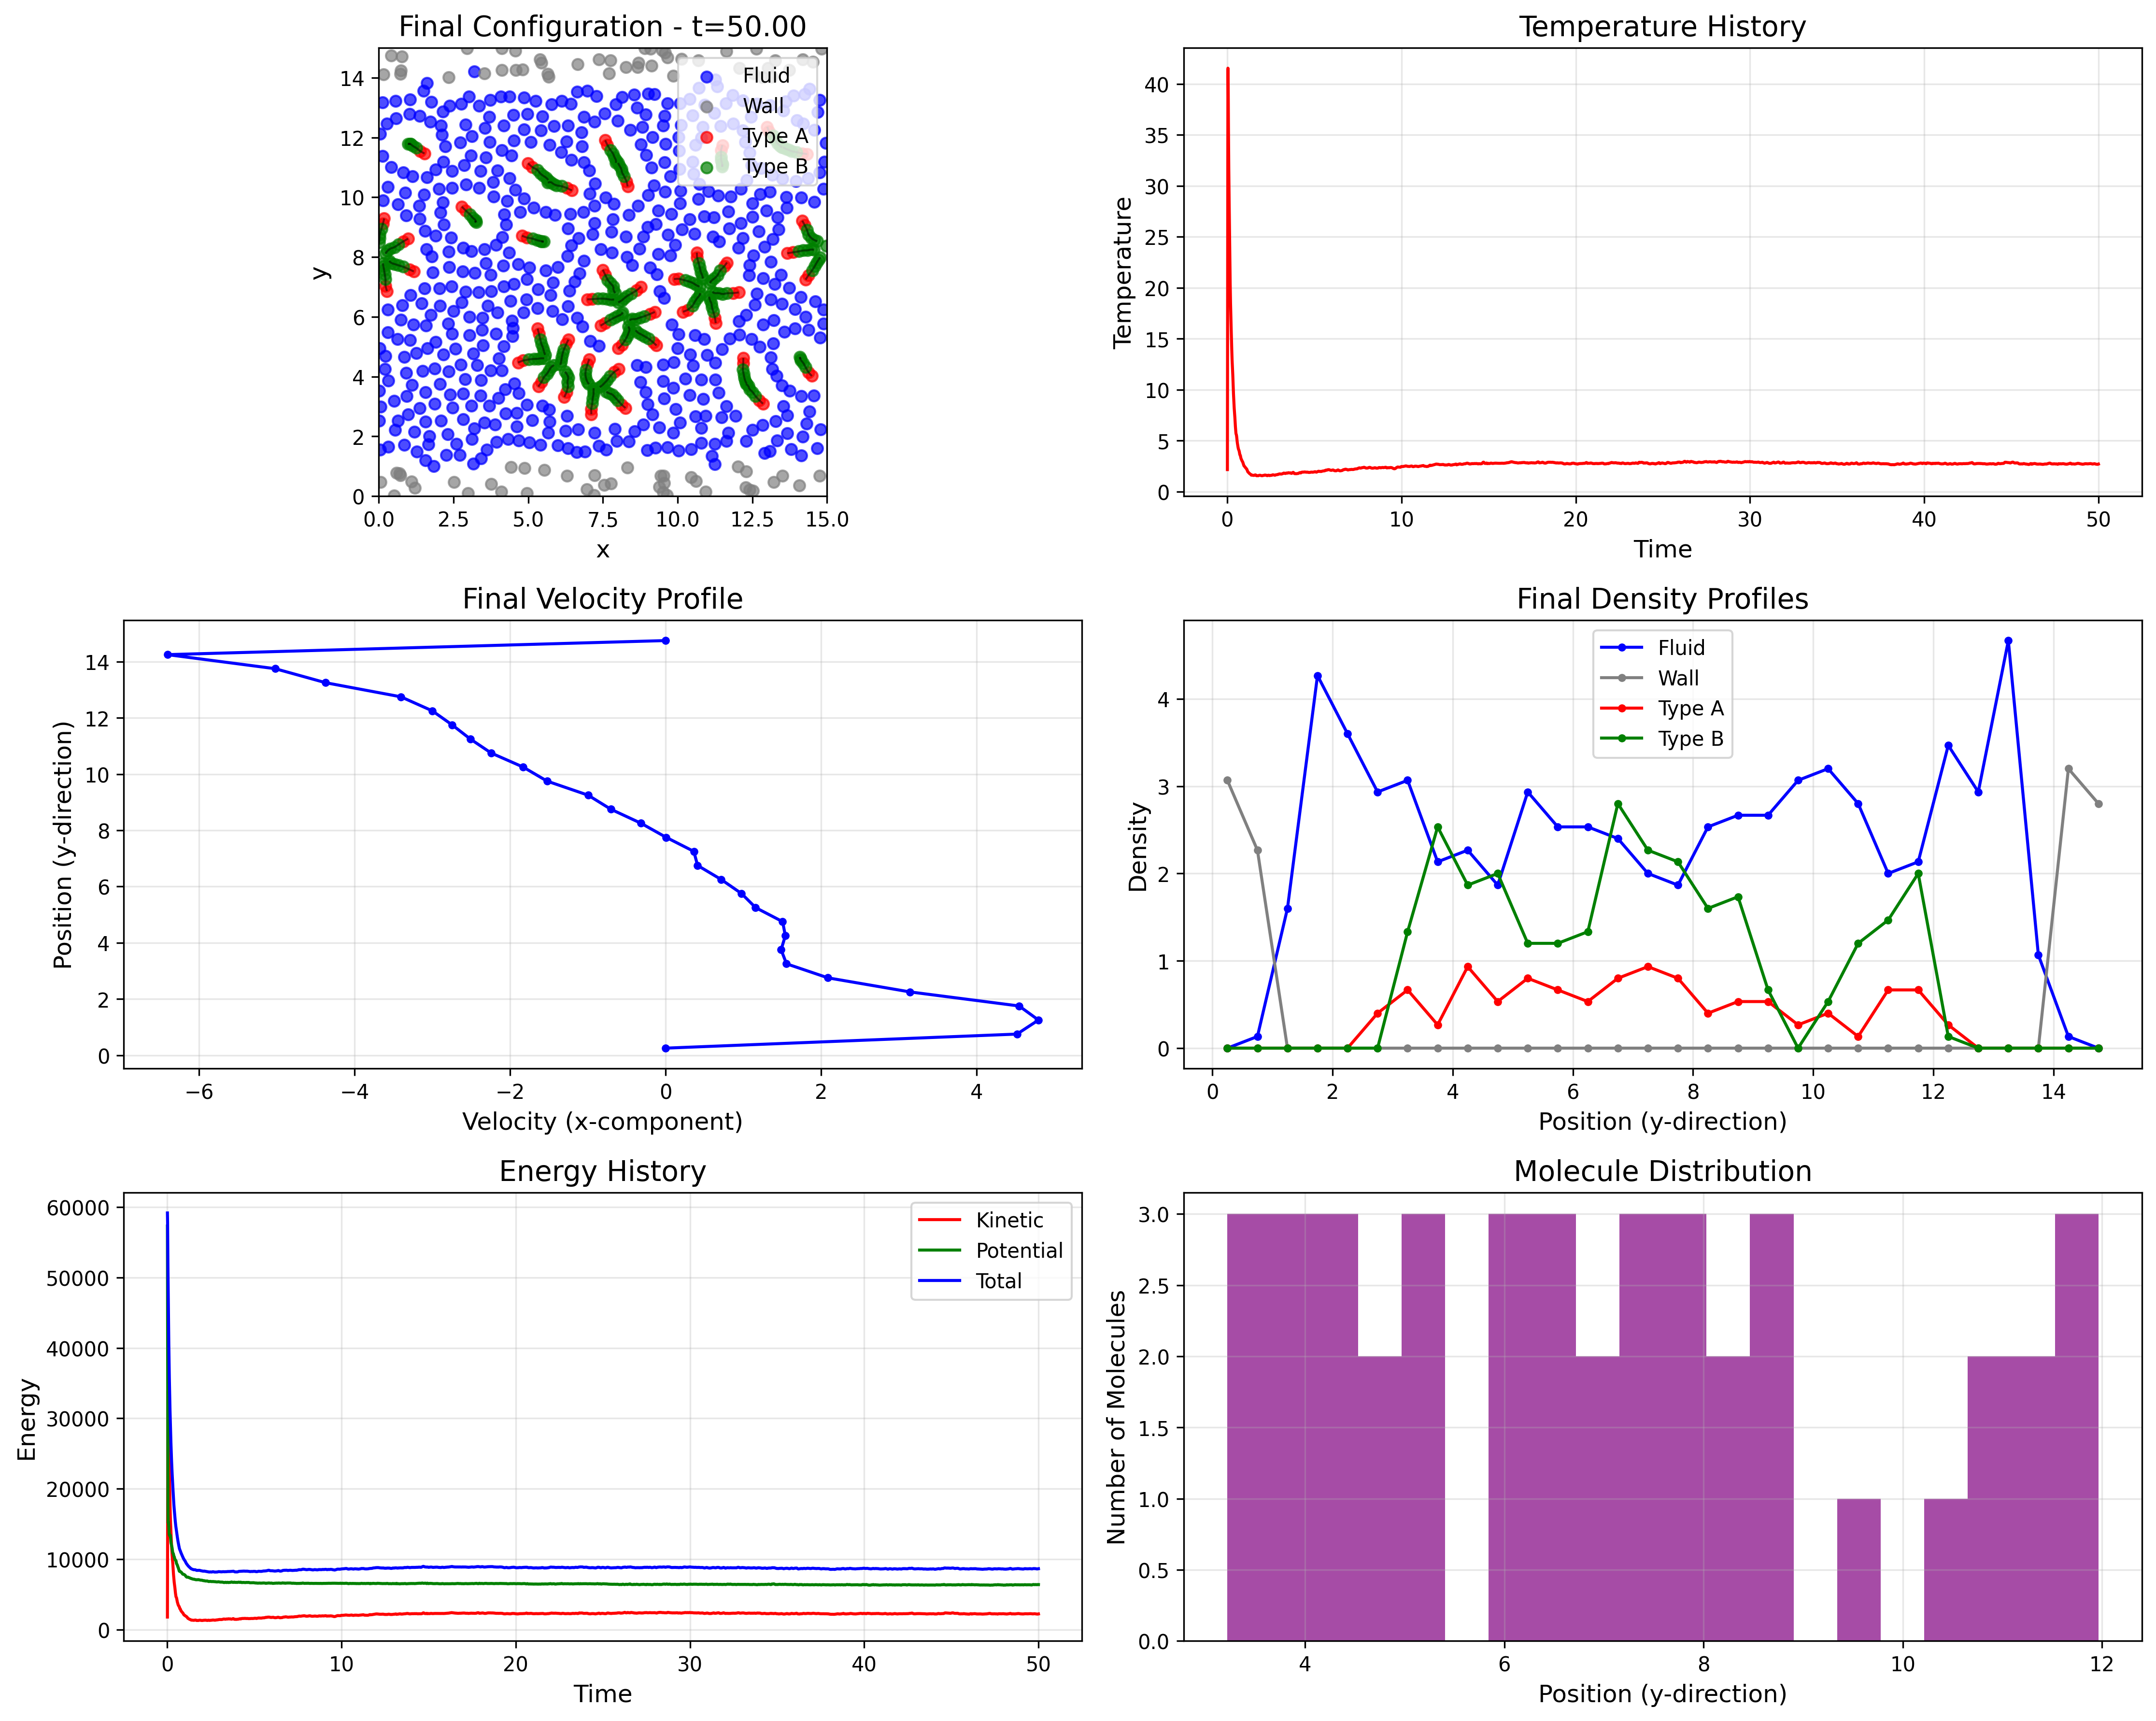
\includegraphics[width=0.95\textwidth]{figures/couette_final_vis.png}
	\end{center}
	\caption{Couette flow with $dt = 0.01$ and $5000$ steps.}\label{fig:couette}
\end{figure}
\subsection{Flow Profile Analysis}
As shown in Figure \ref{fig:couette}, after $5000$ timesteps, the velocity profile demonstrates a nearly linear relationship between position and velocity in the central region of the channel, which is characteristic of Couette flow. Near the walls, there are some deviations from linearity due to the discrete nature of the walls and molecular interactions.
\subsection{Molecule Distribution and Motion}
The chain molecules show interesting behavior in the flow. As visible in the final configuration and molecule distribution histogram:
\begin{enumerate}
	\item The molecules tend to align with the flow direction due to shear forces, with their long axis parallel to the flow.
	\item There is a noticeable depletion of chain molecules near the walls and some concentration in the center region.
	\item The distribution of molecules is not completely uniform across the channel, suggesting preferential positioning.
\end{enumerate}
This behavior can be explained by the interaction parameters. The strong repulsion between type B particles and fluid particles ($a_{BF} = 300$) causes the B-rich chain ends to avoid fluid-dense regions. Additionally, the very weak interaction between B-B particles ($a_{BB} = 1$) allows them to approach each other closely, promoting aggregation of the chains. The walls strongly repel all particle types ($a_{iW} = 200$), creating a depletion layer near the boundaries.
The molecules appear to rotate as they move through the flow, with the shear forces causing them to tumble periodically. This rotation is more pronounced in the center of the channel where the velocity gradient is highest.

